\documentclass[14pt]{extreport}
\usepackage{fontspec}
\usepackage[a4paper,left=25mm,right=10mm,top=15mm,bottom=30mm,footskip=15mm,headsep=5.03978mm]{geometry} % headsep=7.5mm-7pt
\usepackage[colorlinks=true,linkcolor=black,citecolor=black,pdftitle={Квантовый телепортатор. Руководство по эксплуатации},pdfsubject={},pdfkeywords={}]{hyperref}
\usepackage{pdfpages}
\usepackage[english, russian]{babel}    
\usepackage{gostforms}

\renewcommand{\headrulewidth}{0.0mm}

\pagestyle{fancy}
\fancyhf{}
\fancypagestyle{plain}{\fancyhf{}}

\setcounter{secnumdepth}{3}
\setcounter{tocdepth}{3}

\ifdefined\overlaypass
\newcounter{overlaypage}
\setcounter{overlaypage}{1}
\AddToShipoutPicture{\AtPageLowerLeft{\includegraphics[page=\arabic{overlaypage}]{./Form/Form.pdf}\stepcounter{overlaypage}}}
\fi

\begin{document}
\begin{sloppypar}

% Начало титульного листа
\enlargegosttitle
\gosttitle
% TOP
{\strut}
% TOP LEFT
{
УТВЕРЖДЕНО\\
СУИР.21.34352.001-ЛУ
}
% TOP RIGHT
{\strut}
% MIDDLE
{
% \uppercase{Устройство для измерения внутренних диаметров}\\*[14pt]
\begin{center}
    \textbf{Курсовая работа} \\  
    по дисциплине \\
    \textit{"<Электронные устройства систем управления">}
    
    \uppercase{Устройство для измерения внутренних диаметров}
\end{center}
\textbf{Пояснительная записка}\\*[14pt]
\textbf{СУИР.21.34352.001 ПЗ}
}
% BOTTOM LEFT
{\strut}
% BOTTOM RIGHT
{\strut}
% BOTTOM
{\strut}
% Конец титульного листа

\setcounter{page}{2}
\section*{Аннотация}
Необходимо разработать устройство для измерения внутренних диаметров стальных цилиндрических деталей. Исходные данные для проектирования:
\begin{itemize}
    \item диапазон изменения диаметра -- 15-100 мм;
    \item допустимая погрешность измерения -- 2\%;
    \item напряжение питания -- 220В 50 Гц;
    \item максимальная скорость перемещения -- 0.3 м/с;
    \item выходной сигнал устройства -- 16-ти разрядный параллельный код.
\end{itemize}
% % \chapter{Техническое предложение}
% \label{ch:chap2}

\section{Библиографический поиск информации о датчиках, выбранного принципа действия}
В настоящее время наиболее широкое распространение получили датчики приближения, которые помимо своей надежности, имеют широкий ряд преимуществ. Имея сравнительно низкую стоимость, датчики приближения охватывают огромный спектр направленности по своему применению во всех отраслях промышленности. Типичными областями использования емкостных датчиков этого типа являются:
\begin{itemize}
	\item сигнализация заполнения емкостей из пластика или стекла;
	\item контроль уровня заполнения прозрачных упаковок;
	\item сигнализация обрыва обмоточного провода;
	\item регулирование натяжения ленты;
	\item поштучный счет любого вида и др.
\end{itemize}

Емкостные датчики линейных и угловых перемещений являются наиболее распространенными приборами, широко используемыми в машиностроении и на транспорте, строительстве и энергетике, в различных измерительных комплексах.

Обычно емкостный датчик представляет собой плоский или цилиндрический конденсатор, одна из обкладок которого испытывает подвергаемое контролю перемещение, вызывая изменение емкости. Пренебрегая краевыми эффектами, можно выразить емкость для плоского конденсатора следующим образом:
\begin{equation}
	\label{eq:e1}
	C = \frac{\varepsilon \varepsilon_0 S}{d}
\end{equation}

, где \(\varepsilon\) -- относительная диэлектрическая проницаемость среды, заключенной между обкладками, \(S\) -- площадь поверхности рассматриваемых обкладок; \(d\) -- расстояние между обкладками.

Емкостные преобразователи могут быть использованы при измерении различных величин по трем направлениям в зависимости от функциональной связи измеряемой неэлектрической величины со следующими параметрами:
\begin{itemize}
	\item переменной диэлектрической проницаемостью среды \(\varepsilon\);
	\item площадью перекрытия обкладок \(S\);
	\item изменяющимся расстоянием между обкладками \(d\).
\end{itemize}

В первом случае емкостные преобразователи можно применять для анализа состава вещества, поскольку диэлектрическая проницаемость является функцией свойств вещества. Особенно широко емкостные преобразователи этого типа применяются при измерении влажности твердых и жидких тел, уровня жидкости, а также определения геометрических размеров небольших объектов. В большинстве случаев практического использования емкостных преобразователей их естественной входной величиной является геометрическое перемещение электродов относительно друг друга. На основе этого принципа построены датчики линейных и угловых перемещений, приборы измерений усилий, вибраций, скорости и ускорения, датчики приближения, давления и деформации.

Включение емкостного датчика в мостовую схему (рисунок \ref{fig:sensor_scheme}), питаемую от источника повышенной частоты, позволяет зафиксировать изменения емкости на \(0.1\%\).

\begin{figure}[ht]
	\centering
	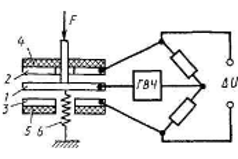
\includegraphics[width=0.5\textwidth]{./images/sensor_scheme.png}
	\caption{Дифференциальный емкостный датчик в мостовой схеме: 1 -- подвижная обкладка; 2-3 -- неподвижные обкладки; 4-5 -- изолирующие прокладки; 6 -- упругий подвес; ГВЧ -- высокочастотный генератор;}
	\label{fig:sensor_scheme}
\end{figure}

Дифференциальный емкостной датчик (рисунок \ref{fig:sensor_scheme}) представляет собой плоский конденсатор с металлической обкладкой 1, на которую действует сила F. Обкладка 1 закреплена на упругой подвеске 6 и под действием силы F перемешается параллельно самой себе.

Две неподвижные обкладки 2 и 3 изолированы от корпуса специальными прокладками 4 и 5. При отсутствии силы F обкладка 1 занимает симметричное положение относительно неподвижных обкладок 2 и 3. При этом емкость конденсатора, образованного пластинами 1 и 2, равна емкости конденсатора, образованного пластинами 1 и 3:
\begin{equation}
	\label{eq:e2}
	C_{1-2} = C_{1-3} = C
\end{equation}

Под воздействием измеряемой силы F, преодолевающей противодействие упругой подвески 6, обкладка 1 перемещается и емкости верхнего и нижнего конденсаторов получают приращения разных знаков:
\begin{equation}
	\label{eq:e3}
	C_{1-2} = C + \Delta C
\end{equation}
\begin{equation}
	\label{eq:e4}
	C_{1-3} = C - \Delta C
\end{equation}

Поскольку эти емкости включены в смежные плечи мостовой схемы; чувствительность измерительной схемы возрастает вдвое. Силы, действующие между парами обкладок, направлены противоположено друг другу, т. е. взаимно компенсируются.

Более высокую чувствительность позволяет получить так называемая резонансная схема. В этом случае емкостный датчик включается в колебательный контур совместно с индуктивным сопротивлением. Резонансная схема показана на рисунке \ref{fig:sensor_scheme2}, а. 
\begin{figure}[ht]
	\centering
	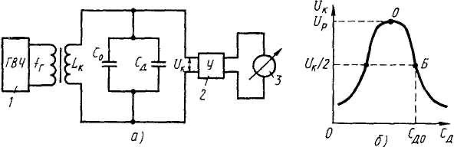
\includegraphics[width=0.66\textwidth]{./images/sensor_scheme2.png}
	\caption{Резонансная измерительная схема включения емкостного датчика: 1 -- высокочастотный генератор; 2 -- усилитель; 3 -- измерительный прибор; \(f_r\) -- частота генератора;}
	\label{fig:sensor_scheme2}
\end{figure}

Высокочастотный генератор 1 имеет частоту напряжения \(f_r\) и питает индуктивно связанный с ним контур, состоящий из индуктивности \(L_k\), подстроечного конденсатора \(C_0\) и емкостного датчика \(C_{d}\). Напряжение \(U_k\), снимаемое с контура, усиливается усилителем 2 и измеряется прибором 3, шкала которого может быть проградуирована в единицах измеряемой величины. При помощи подстроенного конденсатора \(C_0\) контур настраивается на частоту \(f_0\), близкую к частоте генератора.

Для расчета характеристик контура можно использовать следующий формулы резонансной частоты \(f_r\) и добротности \(Q\): 
\begin{equation}
	\label{eq:freq}
	f_r = \frac{1}{2 \pi \sqrt{L_k(C_0 + C_d)}}
\end{equation}
\begin{equation}
	\label{eq:dobr}
	Q = \frac{1}{R} \sqrt{\frac{L_k}{C_0 + C_d}}
\end{equation}
Учитывая, что схема, представленная на рисунке \ref{fig:sensor_scheme2} имеет более высокую чувствительность, то выбираем в качестве емкостного датчика именно её. При этом стоит обратить внимание, что принцип датчиков одинаковый, т.к. они состоят из двух обкладок конденсаторов. То есть важно обеспечить подключение «+» и «-» на каждую из обкладок, выходной информационный сигнал подключим для дальнейшего измерения, а опрос датчика будем проводить с помощью генератора высокочастотного сигнала (ГВЧ).


\section{Разработка функциональной схемы устройства}
Функциональная схема устройства показана на рисунке \ref{fig:func_scheme}. 
\begin{figure}[ht]
	\centering
	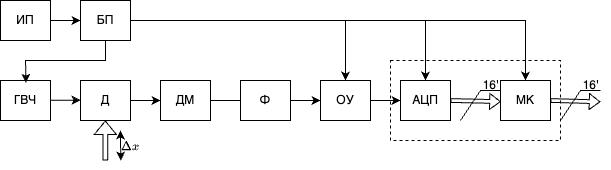
\includegraphics[width=\textwidth]{./images/func_scheme.png}
	\caption{Функциональная схема устройства: ИП -- источник питания; БП -- блок питания; Д -- датчик; ОУ -- операционный усилитель; АЦП -- аналого-цифровой преобразователь; МК -- микроконтроллер; ЭПУ -- электрическое преобразовательное устройство; ГВЧ -- высокочастотный генератор; Ф -- RC-фильтр; МВ -- мостовой выпрямитель;}
	\label{fig:func_scheme}
\end{figure}

В состав функциональной схемы входят:
\begin{enumerate}
	\item Источник питания (ИП) -- промышленная электросеть с параметрами переменного тока 220 В и частотой 50 Гц. Обеспечивает электропитанием все элементы и устройства для измерения внутреннего диаметра;
	\item Блок питания (БП) -- устройство, предназначенное для формирования напряжения питания датчика. Включает в себя стабилизатор напряжения;
	\item Датчик (Д) -- представляет собой емкостной датчик, образованный двумя пластинами, который позволяет проводить измерение внутреннего диаметра;
	\item Операционный усилитель (ОУ) -- усиливает выходной сигнал с датчика до необходимого уровня;
	\item Аналого-цифровой преобразователь (АЦП) -- позволяет преобразовывать аналоговый сигнал измерения диаметра в цифровое значение для его последующей обработки;
	\item Микроконтроллер (МК) -- позволяет проводить обработку сигнала диаметра для последующего использования;
	\item Электрическое преобразовательное устройство (ЭПУ) -- управляемый выпрямитель, преобразующий переменный ток в постоянный с заданными параметрами для питания ОУ, АЦП и МК;
	\item Высокочастотный генератор (ГВЧ) -- генерирует напряжением переменного тока повышенной частоты для Д;
	\item Мостовой выпрямитель (МВ) -- выпрямляет сигнал с Д для обеспечения стабильного постоянного напряжения;
	\item RC-фильтр (Ф) -- фильтрует сигнал с Д для обеспечения сигнала без высокочастотных шумов.
\end{enumerate}

% \subsection{Работа схемы в статике}
% От источника питания поступает переменное напряжение сети (220 В, 50 Гц), которое подаётся на ЭПУ. 
% ЭПУ преобразует переменное напряжение в постоянное 3.3 В, обеспечивая питание МК.
% БП формирует стабильное напряжение 5 В для питания ГВЧ. 
% ГВЧ питает Д, обеспечивая его работу с необходимой частотой.

% Перед подачей сигнала на АЦП, выходной сигнал с операционного усилителя (ОУ) проходит через мостовой выпрямитель и RC-фильтр, что обеспечивает стабильное постоянное напряжение без высокочастотных шумов.
% ОУ усиливает выходной сигнал с датчика до необходимого уровня, после чего АЦП преобразует аналоговый сигнал в цифровой формат для дальнейшей обработки. 
% МК обрабатывает цифровые данные, выполняет необходимые вычисления и формирует 16-ти разрядный параллельный код, представляющий текущее значение измеряемой величины.

% \subsection{Работа схемы в динамике}

При изменении внутреннего диаметра объекта, емкостной датчик (Д) фиксирует изменение емкости \(C_d\) за счет изменения расстояния между обкладками. 
ГВЧ питает датчик переменным током высокой частоты, обеспечивая его работу в колебательном контуре. 
Изменение емкости датчика приводит к изменению параметров колебательного контура, что вызывает изменение выходного сигнала напряжения \(U_k\).

ОУ усиливает этот изменённый сигнал. Перед подачей сигнала на АЦП, выходной сигнал с ОУ проходит через мостовой выпрямитель и RC-фильтр, что обеспечивает стабильное постоянное напряжение без высокочастотных шумов, после чего АЦП преобразует его в цифровой формат. МК обрабатывает цифровые данные, выполняет необходимые вычисления и формирует 16-ти разрядный параллельный код, представляющий текущее значение внутреннего диаметра.
\endinput

\renewcommand\contentsname{\vspace{-32mm}\centerline{\Large{Содержание}}}
\tableofcontents
\newpage

% \chapter{Техническое предложение}
% \label{ch:chap2}

\section{Библиографический поиск информации о датчиках, выбранного принципа действия}
В настоящее время наиболее широкое распространение получили датчики приближения, которые помимо своей надежности, имеют широкий ряд преимуществ. Имея сравнительно низкую стоимость, датчики приближения охватывают огромный спектр направленности по своему применению во всех отраслях промышленности. Типичными областями использования емкостных датчиков этого типа являются:
\begin{itemize}
	\item сигнализация заполнения емкостей из пластика или стекла;
	\item контроль уровня заполнения прозрачных упаковок;
	\item сигнализация обрыва обмоточного провода;
	\item регулирование натяжения ленты;
	\item поштучный счет любого вида и др.
\end{itemize}

Емкостные датчики линейных и угловых перемещений являются наиболее распространенными приборами, широко используемыми в машиностроении и на транспорте, строительстве и энергетике, в различных измерительных комплексах.

Обычно емкостный датчик представляет собой плоский или цилиндрический конденсатор, одна из обкладок которого испытывает подвергаемое контролю перемещение, вызывая изменение емкости. Пренебрегая краевыми эффектами, можно выразить емкость для плоского конденсатора следующим образом:
\begin{equation}
	\label{eq:e1}
	C = \frac{\varepsilon \varepsilon_0 S}{d}
\end{equation}

, где \(\varepsilon\) -- относительная диэлектрическая проницаемость среды, заключенной между обкладками, \(S\) -- площадь поверхности рассматриваемых обкладок; \(d\) -- расстояние между обкладками.

Емкостные преобразователи могут быть использованы при измерении различных величин по трем направлениям в зависимости от функциональной связи измеряемой неэлектрической величины со следующими параметрами:
\begin{itemize}
	\item переменной диэлектрической проницаемостью среды \(\varepsilon\);
	\item площадью перекрытия обкладок \(S\);
	\item изменяющимся расстоянием между обкладками \(d\).
\end{itemize}

В первом случае емкостные преобразователи можно применять для анализа состава вещества, поскольку диэлектрическая проницаемость является функцией свойств вещества. Особенно широко емкостные преобразователи этого типа применяются при измерении влажности твердых и жидких тел, уровня жидкости, а также определения геометрических размеров небольших объектов. В большинстве случаев практического использования емкостных преобразователей их естественной входной величиной является геометрическое перемещение электродов относительно друг друга. На основе этого принципа построены датчики линейных и угловых перемещений, приборы измерений усилий, вибраций, скорости и ускорения, датчики приближения, давления и деформации.

Включение емкостного датчика в мостовую схему (рисунок \ref{fig:sensor_scheme}), питаемую от источника повышенной частоты, позволяет зафиксировать изменения емкости на \(0.1\%\).

\begin{figure}[ht]
	\centering
	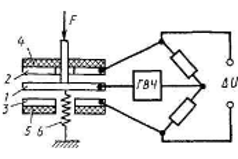
\includegraphics[width=0.5\textwidth]{./images/sensor_scheme.png}
	\caption{Дифференциальный емкостный датчик в мостовой схеме: 1 -- подвижная обкладка; 2-3 -- неподвижные обкладки; 4-5 -- изолирующие прокладки; 6 -- упругий подвес; ГВЧ -- высокочастотный генератор;}
	\label{fig:sensor_scheme}
\end{figure}

Дифференциальный емкостной датчик (рисунок \ref{fig:sensor_scheme}) представляет собой плоский конденсатор с металлической обкладкой 1, на которую действует сила F. Обкладка 1 закреплена на упругой подвеске 6 и под действием силы F перемешается параллельно самой себе.

Две неподвижные обкладки 2 и 3 изолированы от корпуса специальными прокладками 4 и 5. При отсутствии силы F обкладка 1 занимает симметричное положение относительно неподвижных обкладок 2 и 3. При этом емкость конденсатора, образованного пластинами 1 и 2, равна емкости конденсатора, образованного пластинами 1 и 3:
\begin{equation}
	\label{eq:e2}
	C_{1-2} = C_{1-3} = C
\end{equation}

Под воздействием измеряемой силы F, преодолевающей противодействие упругой подвески 6, обкладка 1 перемещается и емкости верхнего и нижнего конденсаторов получают приращения разных знаков:
\begin{equation}
	\label{eq:e3}
	C_{1-2} = C + \Delta C
\end{equation}
\begin{equation}
	\label{eq:e4}
	C_{1-3} = C - \Delta C
\end{equation}

Поскольку эти емкости включены в смежные плечи мостовой схемы; чувствительность измерительной схемы возрастает вдвое. Силы, действующие между парами обкладок, направлены противоположено друг другу, т. е. взаимно компенсируются.

Более высокую чувствительность позволяет получить так называемая резонансная схема. В этом случае емкостный датчик включается в колебательный контур совместно с индуктивным сопротивлением. Резонансная схема показана на рисунке \ref{fig:sensor_scheme2}, а. 
\begin{figure}[ht]
	\centering
	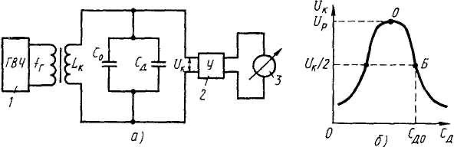
\includegraphics[width=0.66\textwidth]{./images/sensor_scheme2.png}
	\caption{Резонансная измерительная схема включения емкостного датчика: 1 -- высокочастотный генератор; 2 -- усилитель; 3 -- измерительный прибор; \(f_r\) -- частота генератора;}
	\label{fig:sensor_scheme2}
\end{figure}

Высокочастотный генератор 1 имеет частоту напряжения \(f_r\) и питает индуктивно связанный с ним контур, состоящий из индуктивности \(L_k\), подстроечного конденсатора \(C_0\) и емкостного датчика \(C_{d}\). Напряжение \(U_k\), снимаемое с контура, усиливается усилителем 2 и измеряется прибором 3, шкала которого может быть проградуирована в единицах измеряемой величины. При помощи подстроенного конденсатора \(C_0\) контур настраивается на частоту \(f_0\), близкую к частоте генератора.

Для расчета характеристик контура можно использовать следующий формулы резонансной частоты \(f_r\) и добротности \(Q\): 
\begin{equation}
	\label{eq:freq}
	f_r = \frac{1}{2 \pi \sqrt{L_k(C_0 + C_d)}}
\end{equation}
\begin{equation}
	\label{eq:dobr}
	Q = \frac{1}{R} \sqrt{\frac{L_k}{C_0 + C_d}}
\end{equation}
Учитывая, что схема, представленная на рисунке \ref{fig:sensor_scheme2} имеет более высокую чувствительность, то выбираем в качестве емкостного датчика именно её. При этом стоит обратить внимание, что принцип датчиков одинаковый, т.к. они состоят из двух обкладок конденсаторов. То есть важно обеспечить подключение «+» и «-» на каждую из обкладок, выходной информационный сигнал подключим для дальнейшего измерения, а опрос датчика будем проводить с помощью генератора высокочастотного сигнала (ГВЧ).


\section{Разработка функциональной схемы устройства}
Функциональная схема устройства показана на рисунке \ref{fig:func_scheme}. 
\begin{figure}[ht]
	\centering
	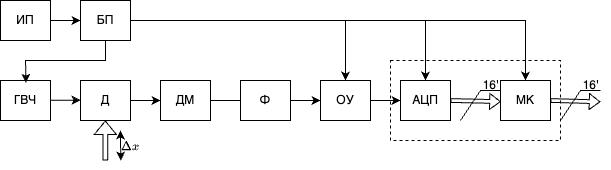
\includegraphics[width=\textwidth]{./images/func_scheme.png}
	\caption{Функциональная схема устройства: ИП -- источник питания; БП -- блок питания; Д -- датчик; ОУ -- операционный усилитель; АЦП -- аналого-цифровой преобразователь; МК -- микроконтроллер; ЭПУ -- электрическое преобразовательное устройство; ГВЧ -- высокочастотный генератор; Ф -- RC-фильтр; МВ -- мостовой выпрямитель;}
	\label{fig:func_scheme}
\end{figure}

В состав функциональной схемы входят:
\begin{enumerate}
	\item Источник питания (ИП) -- промышленная электросеть с параметрами переменного тока 220 В и частотой 50 Гц. Обеспечивает электропитанием все элементы и устройства для измерения внутреннего диаметра;
	\item Блок питания (БП) -- устройство, предназначенное для формирования напряжения питания датчика. Включает в себя стабилизатор напряжения;
	\item Датчик (Д) -- представляет собой емкостной датчик, образованный двумя пластинами, который позволяет проводить измерение внутреннего диаметра;
	\item Операционный усилитель (ОУ) -- усиливает выходной сигнал с датчика до необходимого уровня;
	\item Аналого-цифровой преобразователь (АЦП) -- позволяет преобразовывать аналоговый сигнал измерения диаметра в цифровое значение для его последующей обработки;
	\item Микроконтроллер (МК) -- позволяет проводить обработку сигнала диаметра для последующего использования;
	\item Электрическое преобразовательное устройство (ЭПУ) -- управляемый выпрямитель, преобразующий переменный ток в постоянный с заданными параметрами для питания ОУ, АЦП и МК;
	\item Высокочастотный генератор (ГВЧ) -- генерирует напряжением переменного тока повышенной частоты для Д;
	\item Мостовой выпрямитель (МВ) -- выпрямляет сигнал с Д для обеспечения стабильного постоянного напряжения;
	\item RC-фильтр (Ф) -- фильтрует сигнал с Д для обеспечения сигнала без высокочастотных шумов.
\end{enumerate}

% \subsection{Работа схемы в статике}
% От источника питания поступает переменное напряжение сети (220 В, 50 Гц), которое подаётся на ЭПУ. 
% ЭПУ преобразует переменное напряжение в постоянное 3.3 В, обеспечивая питание МК.
% БП формирует стабильное напряжение 5 В для питания ГВЧ. 
% ГВЧ питает Д, обеспечивая его работу с необходимой частотой.

% Перед подачей сигнала на АЦП, выходной сигнал с операционного усилителя (ОУ) проходит через мостовой выпрямитель и RC-фильтр, что обеспечивает стабильное постоянное напряжение без высокочастотных шумов.
% ОУ усиливает выходной сигнал с датчика до необходимого уровня, после чего АЦП преобразует аналоговый сигнал в цифровой формат для дальнейшей обработки. 
% МК обрабатывает цифровые данные, выполняет необходимые вычисления и формирует 16-ти разрядный параллельный код, представляющий текущее значение измеряемой величины.

% \subsection{Работа схемы в динамике}

При изменении внутреннего диаметра объекта, емкостной датчик (Д) фиксирует изменение емкости \(C_d\) за счет изменения расстояния между обкладками. 
ГВЧ питает датчик переменным током высокой частоты, обеспечивая его работу в колебательном контуре. 
Изменение емкости датчика приводит к изменению параметров колебательного контура, что вызывает изменение выходного сигнала напряжения \(U_k\).

ОУ усиливает этот изменённый сигнал. Перед подачей сигнала на АЦП, выходной сигнал с ОУ проходит через мостовой выпрямитель и RC-фильтр, что обеспечивает стабильное постоянное напряжение без высокочастотных шумов, после чего АЦП преобразует его в цифровой формат. МК обрабатывает цифровые данные, выполняет необходимые вычисления и формирует 16-ти разрядный параллельный код, представляющий текущее значение внутреннего диаметра.
\endinput
% \chapter{Разработка собственного технического решения}
% \label{ch:chap3}

\section{Разработка принципиальной электрической схемы (или схемы соединений) вторичного преобразователя}
Принципиальная электрическая схема разрабатывается на основании анализа исходных данных и принятой функциональной схемы (рисунок \ref{fig:func_scheme}). Задача разработки электрической схемы проектируемого устройства заключается в выборе и обосновании принципиальных схем каскадов для реализации структурной схемы.

Вначале произведем анализ известных схемных решений проектируемого каскада. Критерии для разрабатываемой схемы: простота, надежность, дешевизна при выполнении заданных требований.

Исходя из разработанной функциональной схемы устройства принципиальная схема состоит из следующих функциональных узлов:
\begin{itemize}
    \item микроконтроллер (включает в себя АЦП);
    \item операционный усилитель;
    \item генератор высоких частот;
    \item блок питания;
    \item управляемый выпрямитель;
    \item RC-фильтр;
    \item емкостной датчик;
\end{itemize}

\newpage
\subsection{Микроконтроллер}
В качестве управляющего устройства выбран микроконтроллер ATmega8 (приложение \ref{appendmk}), использующийся в Arduino. Условное графическое обозначение микроконтроллера изображено
на рисунке \ref{fig:mk}.
\begin{figure}[ht]
	\centering
	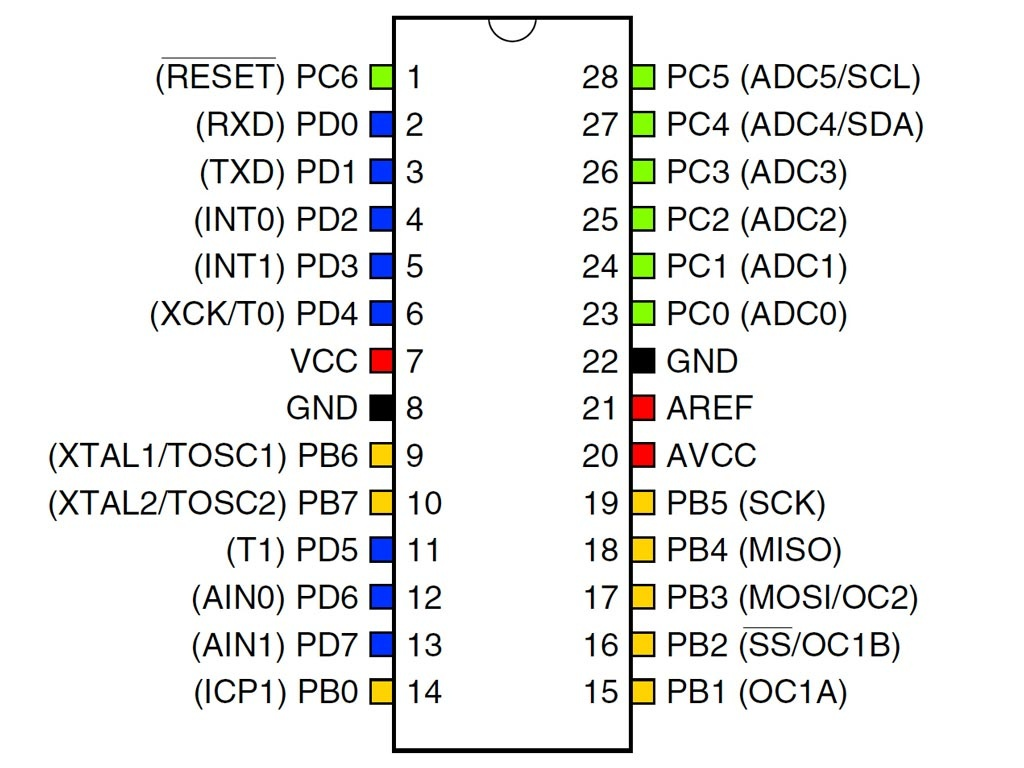
\includegraphics[width=0.6\textwidth]{./images/mk.png}
	\caption{Микроконтроллер ATmega8}
	\label{fig:mk}
\end{figure}
Характеристики:
\begin{itemize}
    \item Напряжение питания: 4.5…5.5 В;
    \item Ширина шины данных: 8-бит;
    \item Тактовая частота:	16 МГц;
    \item Количество входов/выходов: 23;
    \item Объем памяти программ: 8 кбайт;
    \item Тип памяти программ: flash;
    \item Встроенные интерфейсы: i2c, spi, uart;
    \item Напряжение питания: 4.5…5.5;
    \item Вес: 4 г;
    \item Наличие АЦП/ЦАП: да;
\end{itemize}
Микроконтроллер уже содержит в себе АЦП и может
давать на выход 16-битный параллельный код, а следовательно, не
требуется производить дополнительных преобразований выходного сигнала.


\subsection{Емкостной датчик}
Датчик собранный по схеме рисунка \ref{fig:sensor_scheme2}. Номиналы компонент датчика:
\(C_0 = 100\)пФ; \(C_d = 47\)пФ; \(L_k = 33\)мГн; \(R=510\)Ом.
Тогда контур обладает резонансной частотой 100КГц и добротностью 0.1. При напряжении питания генератора частот 15В ожидается уровень выходного сигнала порядка 1.5В.


\subsection{Операционный усилитель}
В схему требуется включить операционный усилитель, предназначенный для усиления аналогового сигнала. Выберем неинвертирующую схему усиления, поскольку в разрабатываемой принципиальной схеме отрицательные полуволны входного напряжения будут выпрямлены выпрямителем на входе схемы. Был выбран LM358 (приложение \ref{appendmult}).

\begin{figure}[ht]
	\centering
	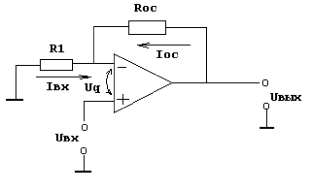
\includegraphics[width=0.6\textwidth]{./images/multiplier.png}
	\caption{Усилитель напряжения}
	\label{fig:multiplier}
\end{figure}
Коэффициент усиления представленной схемы рассчитывается по формуле \ref{eq:multiplier}.
\begin{equation}
    \label{eq:multiplier}
    \frac{U_{out}}{U_{in}} = \frac{R_{2} + R_1}{R_1} = 3
\end{equation}
Сигнал с датчика составляет порядка 1.5 В, а для работы микроконтроллера необходимо уровень от 2,6 до 5 В. 
Возьмем \(R_1 = 1\) кОм и \(R_2 = 2\) кОм, тогда коэффициент усиления равен~3.

\subsection{Генератор высоких частот}

В качестве генератора высоких частот был выбран EGP Proever XR2206 (приложение \ref{appendgenerator}). Требуемое питание 12 В, диапазон генерируемых частот 1Гц -- 1МГц. Обладает гибкой регулировкой, а так же несколькими режимами работы. Генератор будет работать с частотой 100 КГц, чтобы совпадать с резонансной частотой датчика.

\subsection{Блок питания}
Импульсный источник питания Mean Well RD-50A (приложение \ref{appendbp}). Блок питания с входным напряжением 220 В AC и выходными напряжениями 5 В DC (для МК) и 12 В DC (для ГВЧ), обеспечивающий стабильное питание компонентов устройства.

\subsection{RC-фильтр}
Длч фильтрации данных с датчика будем использовать RC-фильтр (рисунок \ref{fig:filter}). АЧХ такого фильтра беспрепятственно пропускает низкие частоты.
\begin{figure}[ht]
	\centering
	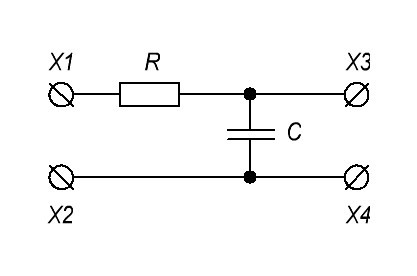
\includegraphics[width=0.6\textwidth]{./images/RC_filt.jpg}
	\caption{Схема RC-фильтра}
	\label{fig:filter}
\end{figure}
Частота среза рассчитывается по формуле
\begin{equation}
    \label{eq:filter}
    f_{c} = \frac{1}{2 \pi R_3 C_3}
\end{equation}
Частота среза должна быть 100кГц, потому что с такой частотой колеблется контур. В следствии этого были выбраны номиналы \(C_3 = 10\)нФ, \(R_3 = 1.6\)КОм.

\newpage
\section{Чертеж Э3 или Э4}
Чертеж представлен в СУИР.21.34352.001 Э3.
% \begin{figure}[ht]
% 	\centering
% 	\includegraphics[width=\textwidth]{./images/scheme.pdf}
% 	\caption{Схема подключения к МК: ИП -- источник питания; Д -- датчик; Z1 -- кварцевый ГВЧ; VD1...4 диоды; C1...C3 -- конденсаторы; R1...R4 -- резисторы; ОУ -- операционный усилитель;}
% 	\label{fig:pr_scheme}
% \end{figure}

На электрической схеме показан источник питания G1 подключен к сети AC 220В 50Гц и дает на выход два канала DC 5В и 12В.

Напряжение с 5В канала блока питания подается на микроконтроллер DD1. На базе элемента ZQ1 с конденсаторами С1 и С2 построен генератор тактовых сигналов. Он необходим для того, чтобы осуществлять работу микроконтроллера на постоянной частоте. Подключение осуществляется в порты XTAL1 и XTAL2 согласно схеме подключения выбранного микроконтроллера.

Напряжение с 12В канала блока питания подается на высокочастотный генератор DA1, который необходим для работы емкостного датчика. После этого сигнал с него идет на датчик DA2, выходом которого является напряжение порядка 1.5В, которое нам нужно измерить. Оно последовательно подается на диодный мост и RC-фильтр, состоящий из \(R_3\) и \(C_3\), после чего усиливается усилителем DA3 в 3 раза и подается на АЦП микроконтроллера PC5.

После этого микроконтроллер готов отдавать полученные значения в 16 битном формате. Для этого выделены порты [PD0...PD7] (старший байт), [PB0...PB5 PC0 PC1] (младший байт), PC3 (синхронизация) и GND. 

Перечень элементов представлен в СУИР.21.34352.001 ПЭ3.
\endinput
\newpage
\section*{Заключение}
В результате выполнения комплексной работы было спроектировано устройство для измерения внутренних диаметров стальных цилиндрических деталей, которое содержит в своём составе емкостной чувствительный элемнент. Устройство обеспечивает измерение диаметра в пределах 15-100 мм и выходной сигнал - 16-ти разрядный параллельный код, что соответствует требованиям технического задания. Работа содержит перечень требуемых компонентов для реализации схемы, а также принципиальную электрическую схему разработанного устройства. 

\newpage
\appendix
% \makeatletter
\titleformat{\chapter}[display]
  {\normalfont\Large\bfseries}
  {\raggedright Приложение\ \thechapter}
  {0pt}{\Large\raggedright}
\titlespacing*{\chapter}{0pt}{0pt}{0pt}
\renewcommand{\thechapter}{\Asbuk{chapter}}

\chapter{Документация к ATmega8}
\label{appendmk}
\begin{figure}[ht]
	\centering
	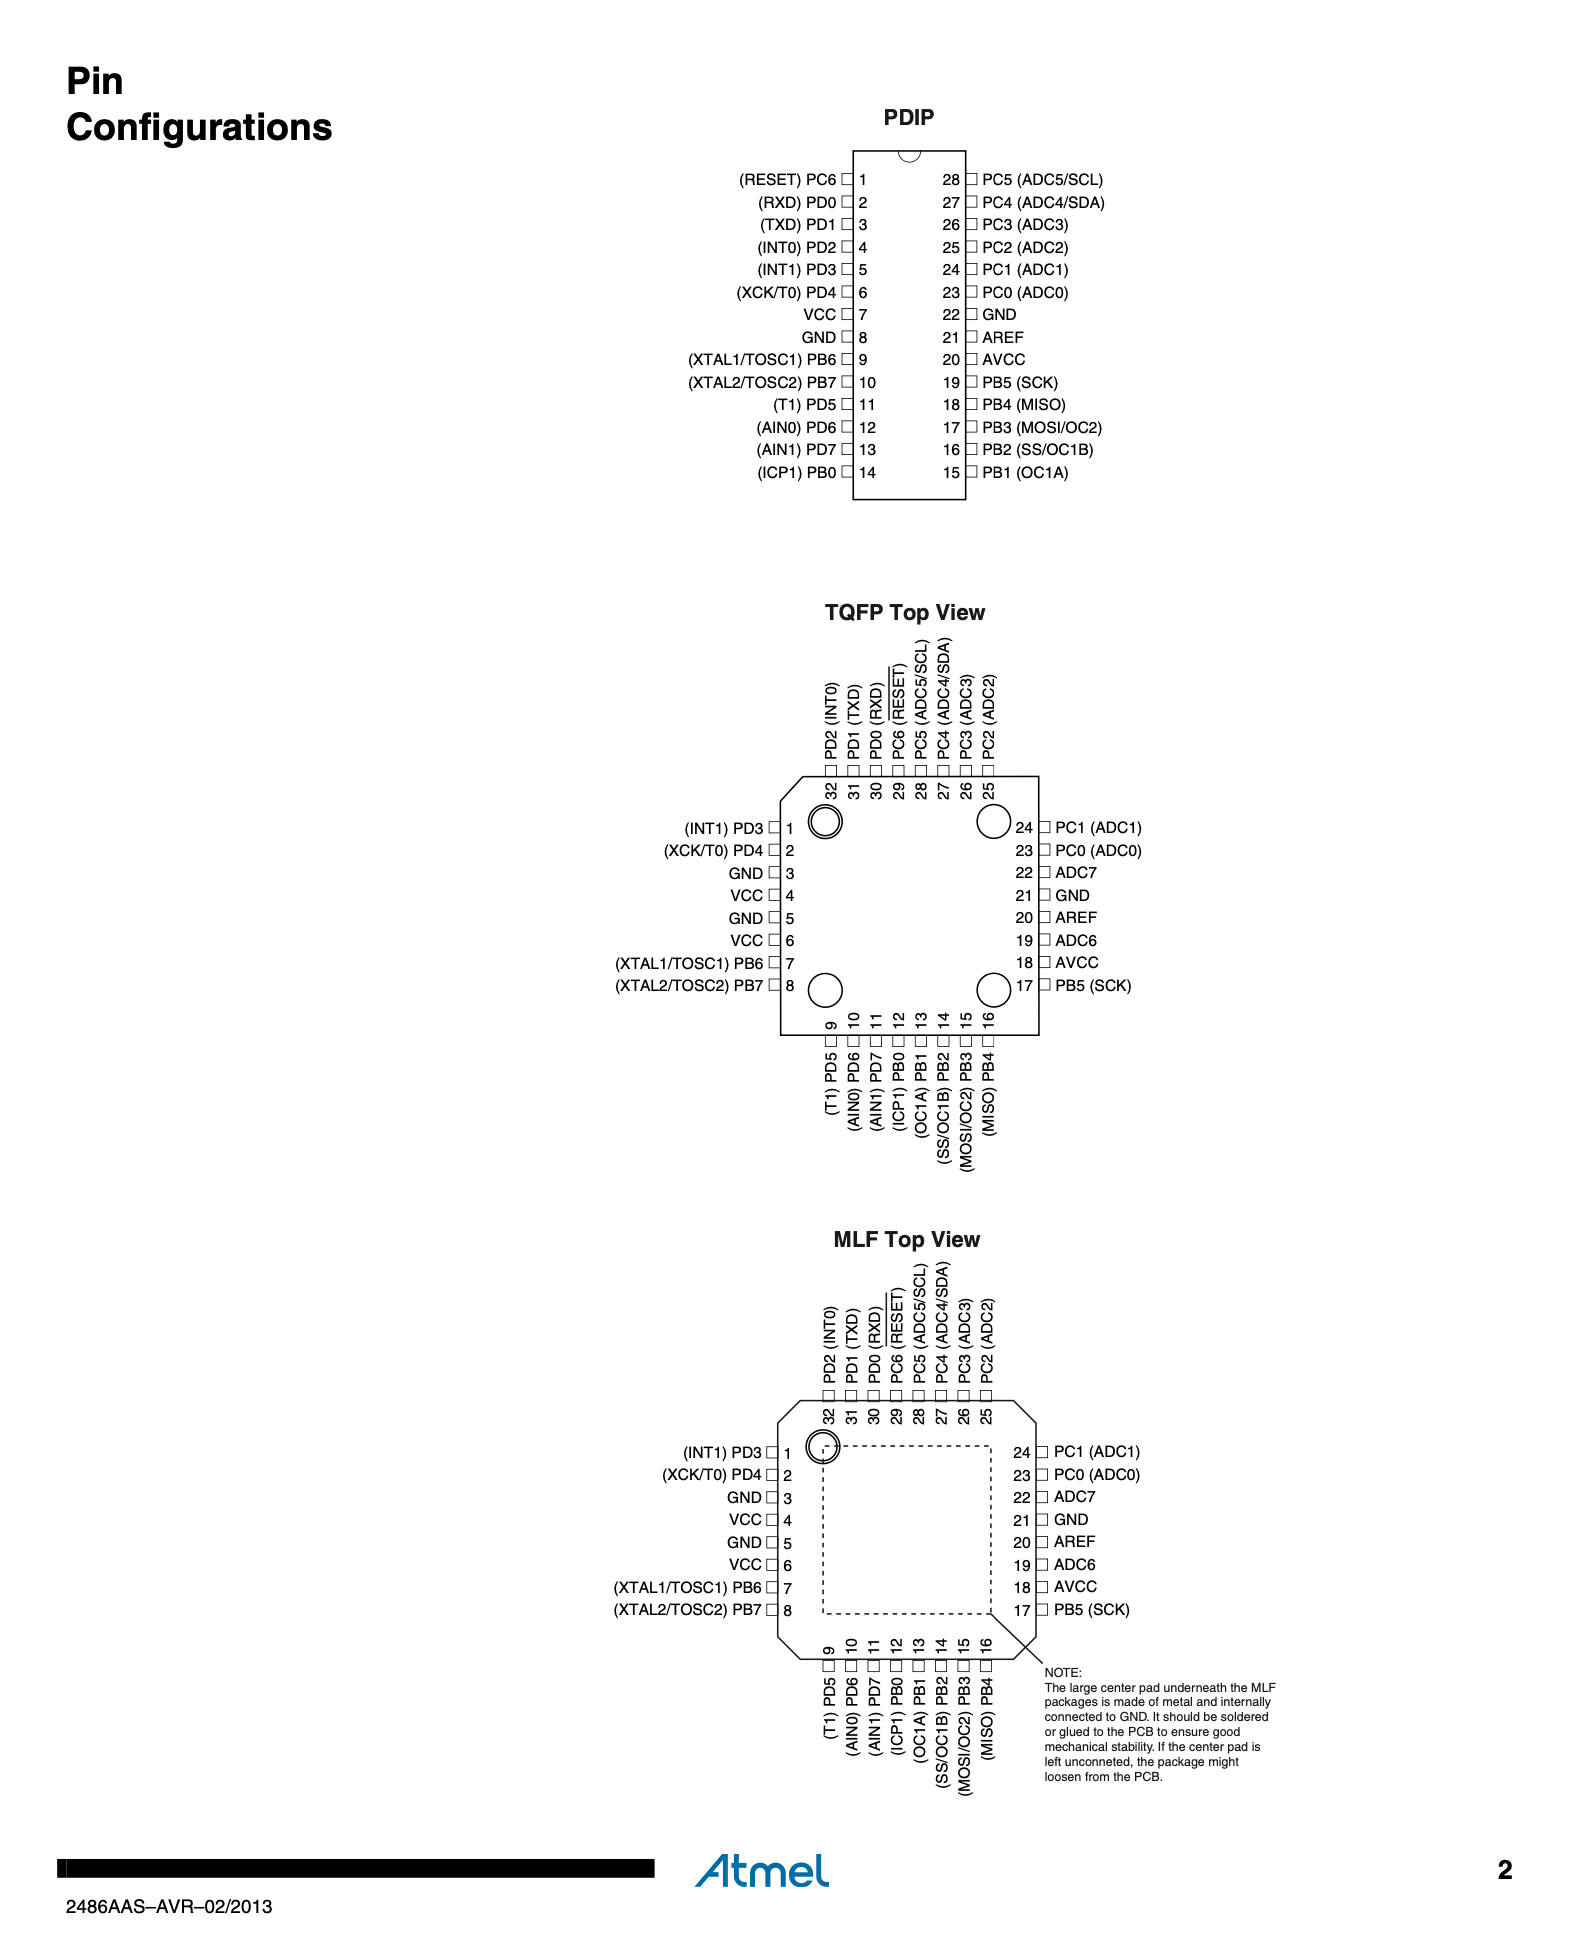
\includegraphics[width=0.9\textwidth]{./images/atmega_dh1.png}
	% \caption{Функциональная схема устройства: ИП -- источник питания; БП -- блок питания; Д -- датчик; ОУ -- операционный усилитель; АЦП -- аналого-цифровой преобразователь; МК -- микроконтроллер; ЭПУ -- электрическое преобразовательное устройство; ГВЧ -- высокочастотный генератор; Ф -- RC-фильтр; МВ -- мостовой выпрямитель;}
	\label{fig:atmega}
\end{figure}
\begin{figure}[ht]
	\centering
	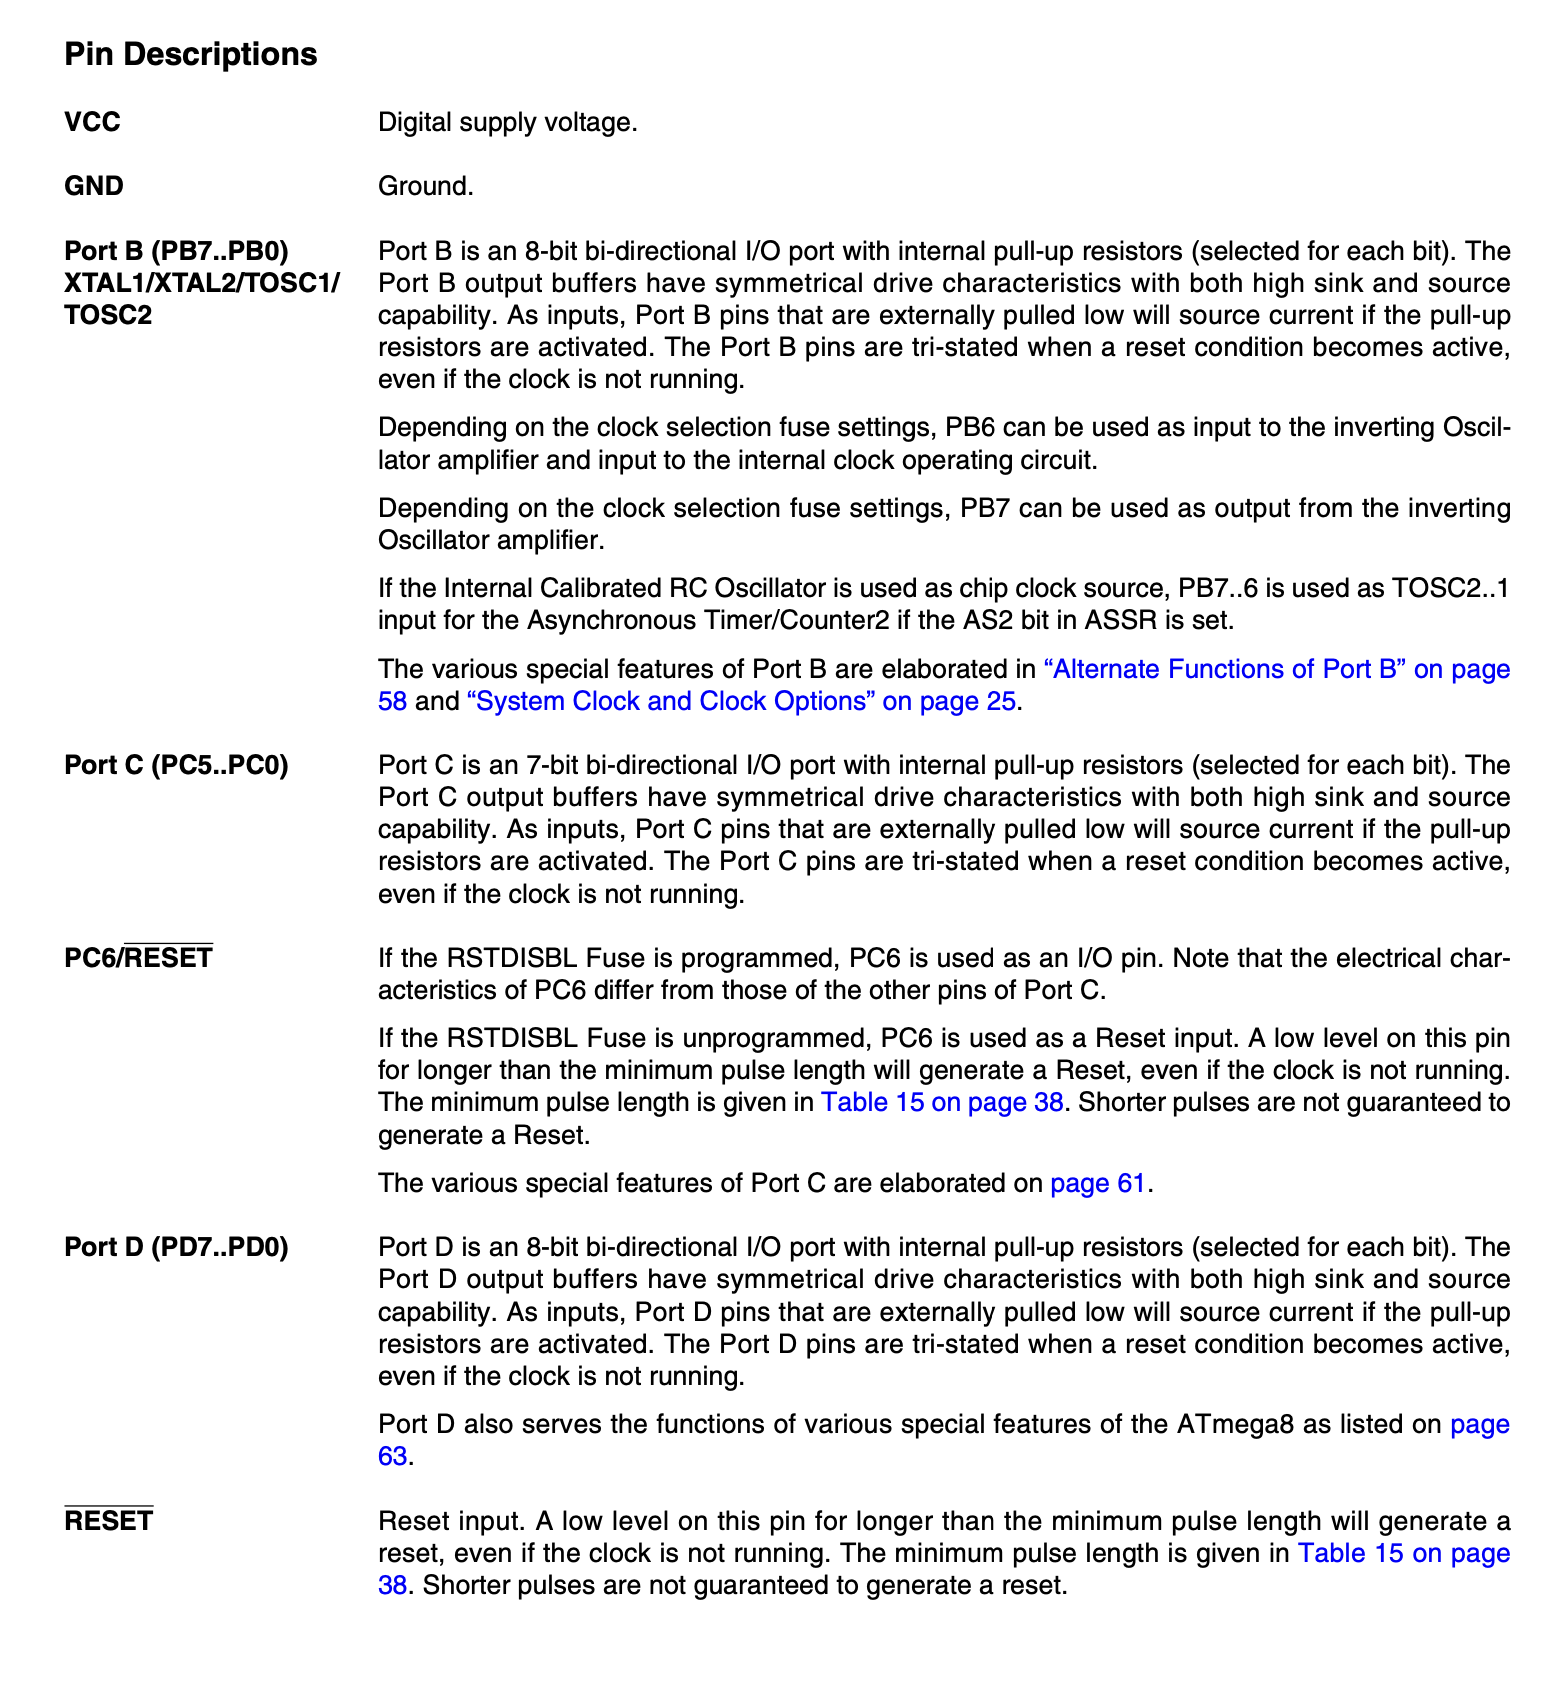
\includegraphics[width=\textwidth]{./images/atmega_dh2.png}
	% \caption{Функциональная схема устройства: ИП -- источник питания; БП -- блок питания; Д -- датчик; ОУ -- операционный усилитель; АЦП -- аналого-цифровой преобразователь; МК -- микроконтроллер; ЭПУ -- электрическое преобразовательное устройство; ГВЧ -- высокочастотный генератор; Ф -- RC-фильтр; МВ -- мостовой выпрямитель;}
	\label{fig:atmega2}
\end{figure}


\chapter{Документация к операционному усилителю}
\label{appendmult}
\begin{figure}[ht]
	\centering
	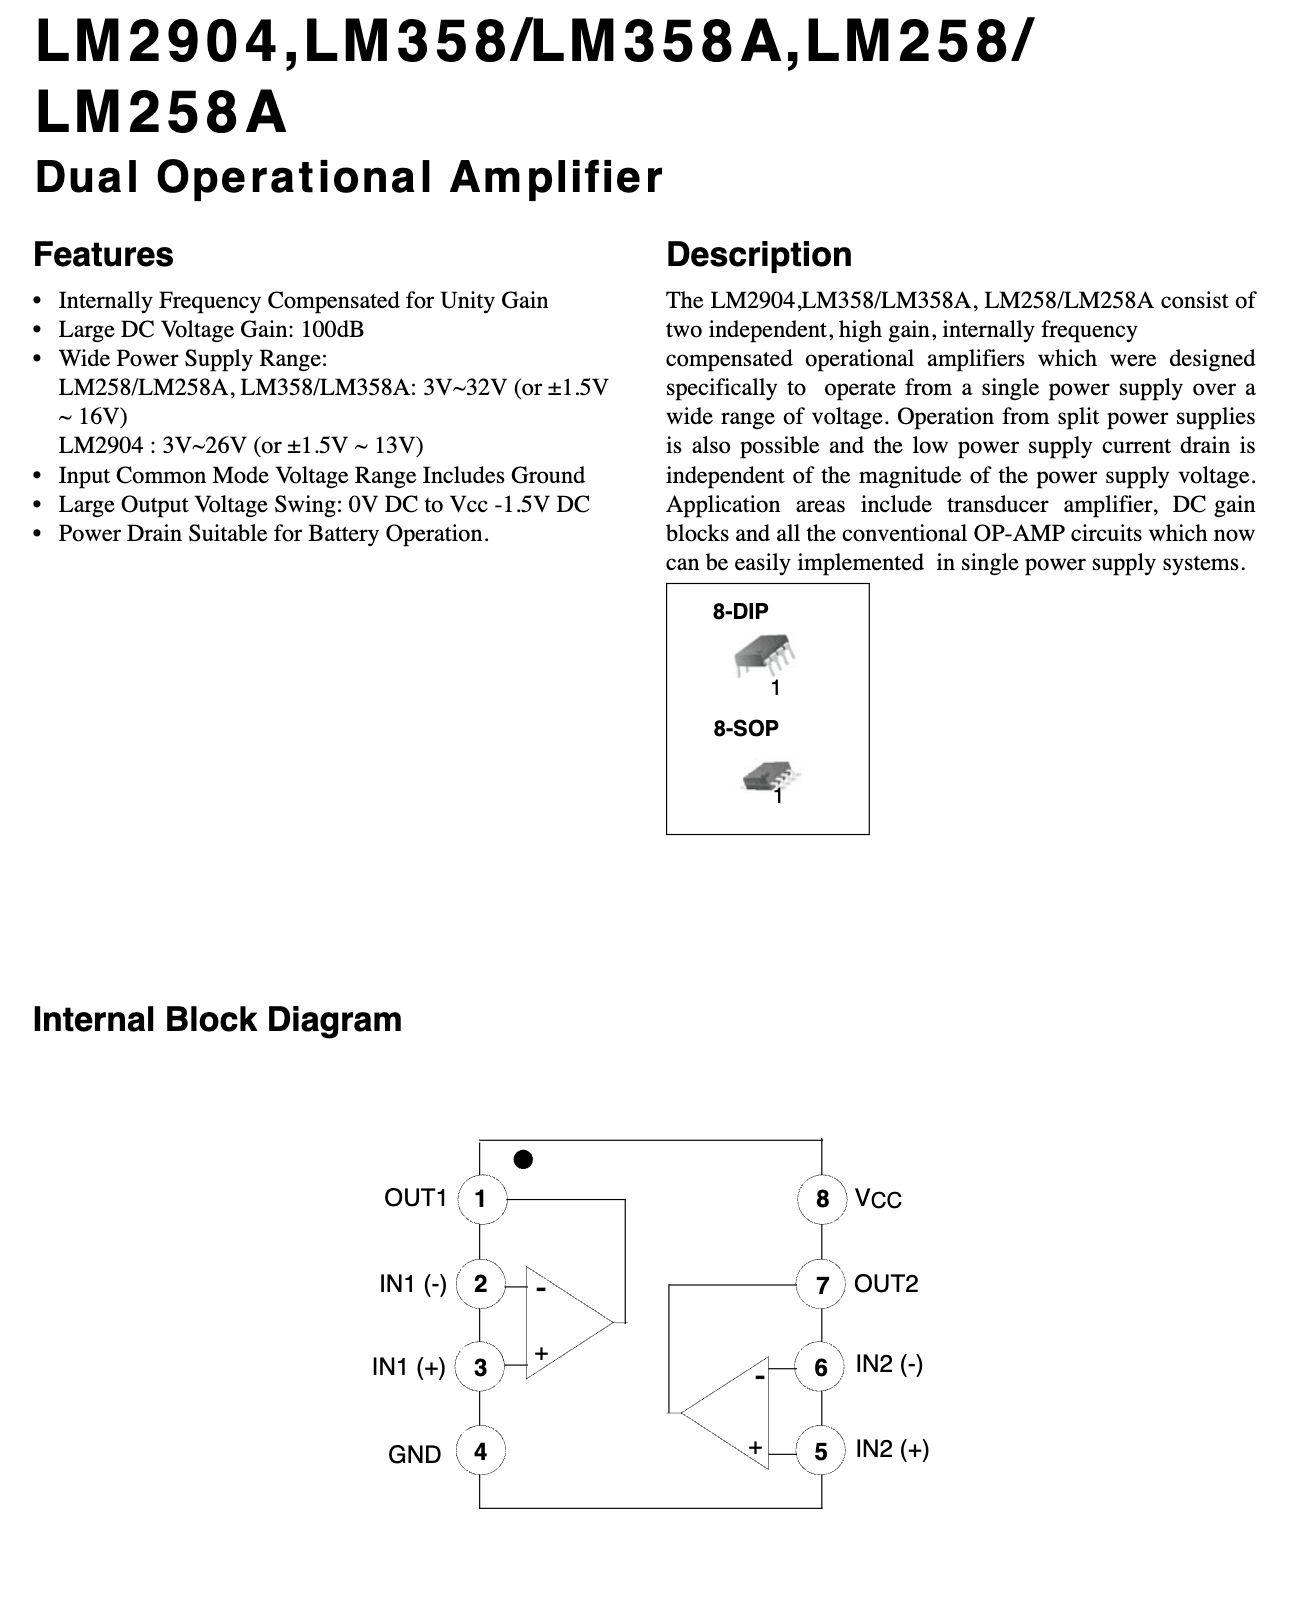
\includegraphics[width=0.8\textwidth]{./images/ou.png}
	% \caption{Функциональная схема устройства: ИП -- источник питания; БП -- блок питания; Д -- датчик; ОУ -- операционный усилитель; АЦП -- аналого-цифровой преобразователь; МК -- микроконтроллер; ЭПУ -- электрическое преобразовательное устройство; ГВЧ -- высокочастотный генератор; Ф -- RC-фильтр; МВ -- мостовой выпрямитель;}
	\label{fig:ou}
\end{figure}


\chapter{Документация к ГВЧ}
\label{appendgenerator}
\begin{figure}[ht]
	\centering
	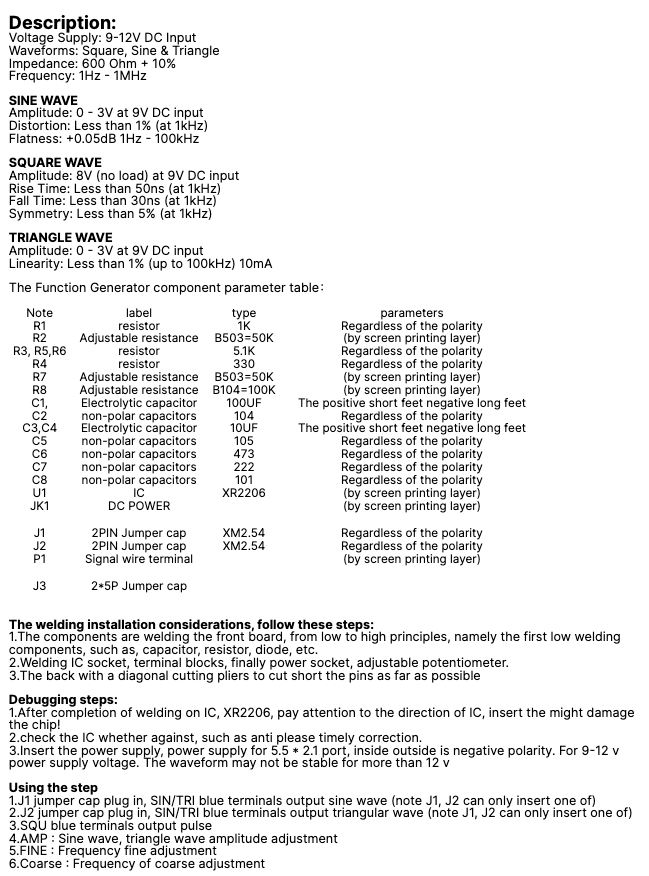
\includegraphics[width=0.8\textwidth]{./images/generator.png}
	% \caption{Функциональная схема устройства: ИП -- источник питания; БП -- блок питания; Д -- датчик; ОУ -- операционный усилитель; АЦП -- аналого-цифровой преобразователь; МК -- микроконтроллер; ЭПУ -- электрическое преобразовательное устройство; ГВЧ -- высокочастотный генератор; Ф -- RC-фильтр; МВ -- мостовой выпрямитель;}
	\label{fig:generator}
\end{figure}


\chapter{Документация к блоку питания}
\label{appendbp}
\begin{figure}[ht]
	\centering
	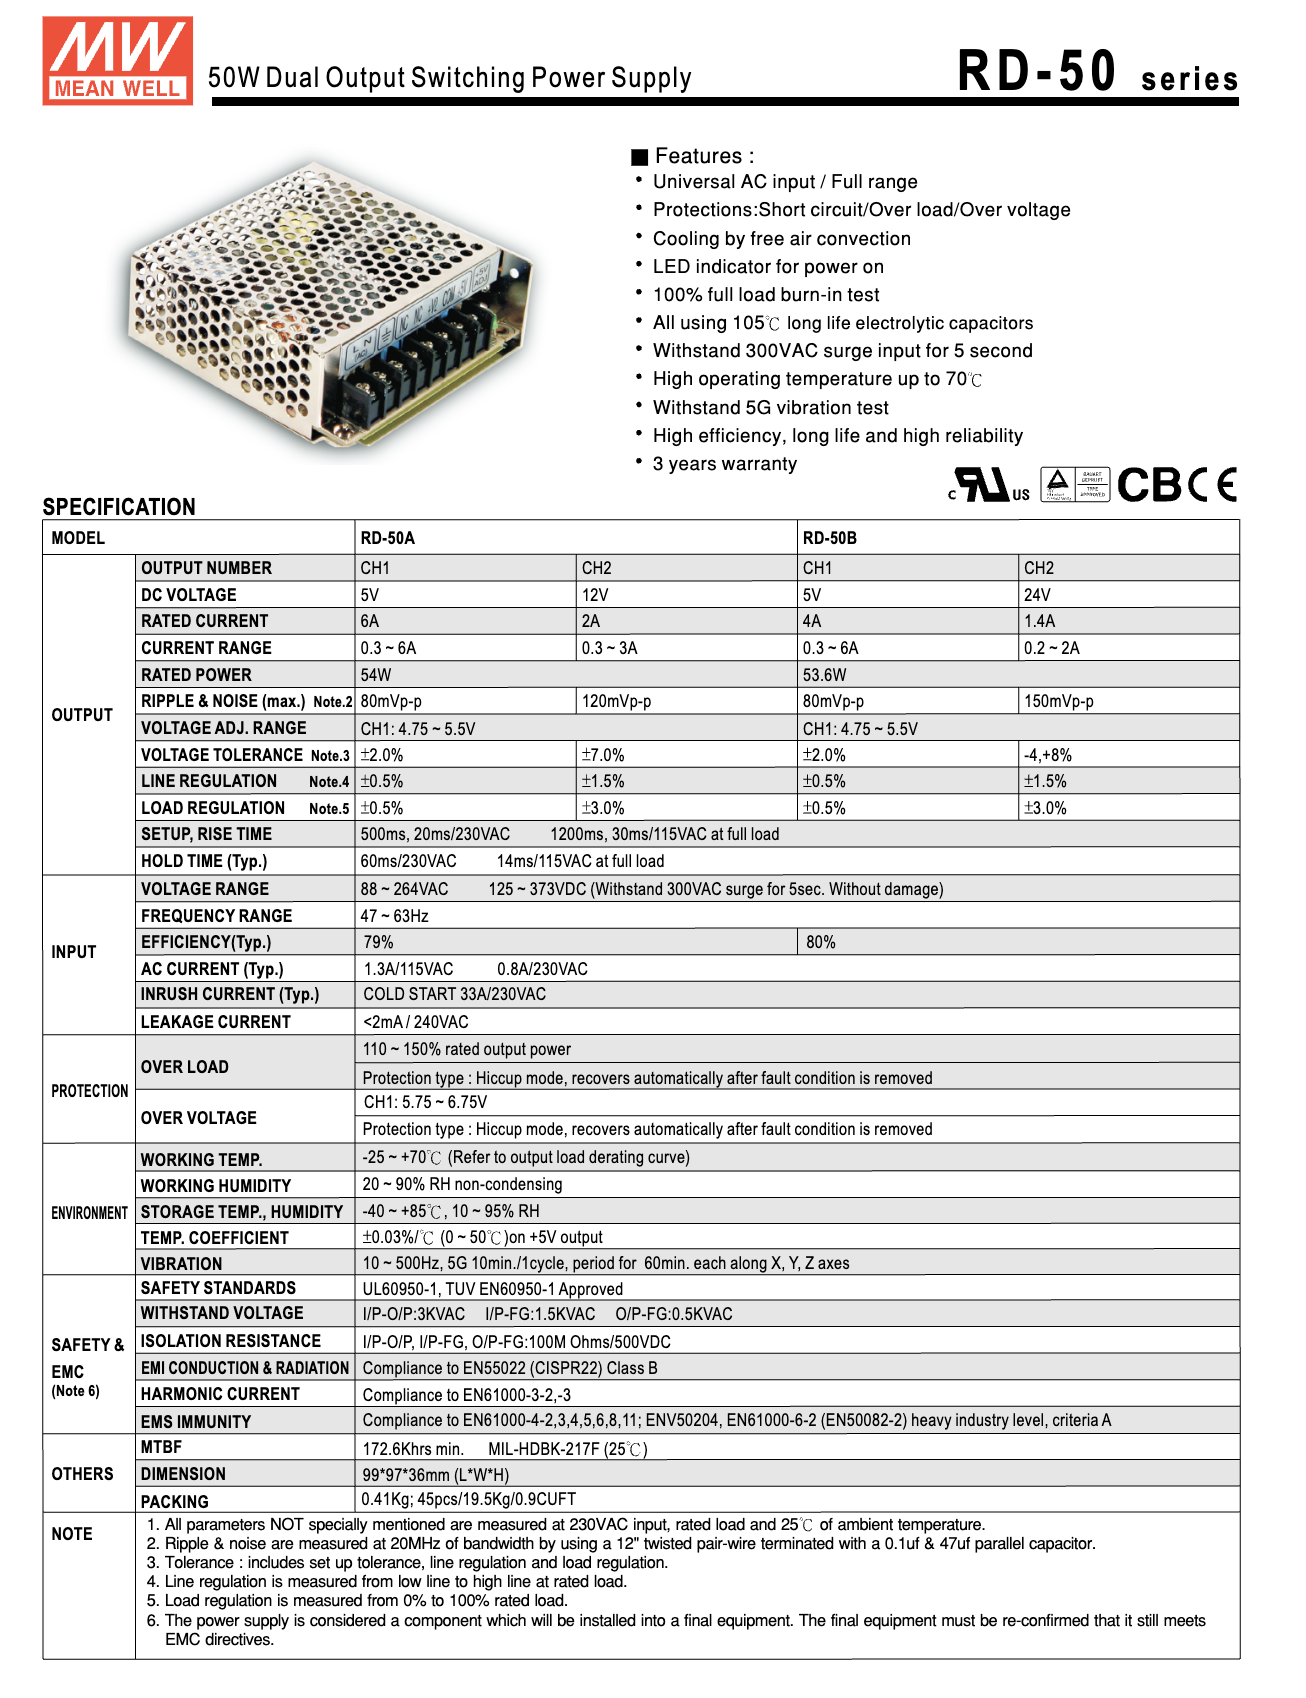
\includegraphics[width=0.9\textwidth]{./images/bp.png}
	% \caption{Функциональная схема устройства: ИП -- источник питания; БП -- блок питания; Д -- датчик; ОУ -- операционный усилитель; АЦП -- аналого-цифровой преобразователь; МК -- микроконтроллер; ЭПУ -- электрическое преобразовательное устройство; ГВЧ -- высокочастотный генератор; Ф -- RC-фильтр; МВ -- мостовой выпрямитель;}
	\label{fig:bp1}
\end{figure}



\end{sloppypar}
\end{document}
